% dimensions(x) returns number of spatial dimensions
% y = transform(x, "proj4string")
% bbox(x)
% coordinates(x) ; <-
% rings(x) ; <-
% method to retrieve lines? --> Lines()?
% gridded(x)  ; <-
% 
\documentclass{article}
% \VignetteIndexEntry{sp: classes and methods for spatial data}

\usepackage{graphicx}
\usepackage[colorlinks=true,urlcolor=blue]{hyperref}

\usepackage{color}

\usepackage{Sweave}
\newcommand{\strong}[1]{{\normalfont\fontseries{b}\selectfont #1}}
\let\pkg=\strong

\title{ S Classes and Methods for Spatial Data:\\
the {\tt sp} Package }
\author{Edzer J.\ Pebesma\footnote{Dept of Physical Geography,
Faculty of Geosciences, Utrecht University, P.O. Box 80.115,
3508 TC Utrecht, The Netherlands {\tt e.pebesma@geo.uu.nl}} \and 
Roger S.\ Bivand\footnote{Economic Geography Section, Department of Economics, %
Norwegian School of Economics and Business Administration, %
Breiviksveien 40, N-5045 Bergen, Norway; {\tt Roger.Bivand@nhh.no}}}
\date{Feb 2005}

\begin{document}

\maketitle
\tableofcontents

\section{Introduction}

The {\tt sp} package provides classes and methods for dealing with
spatial data in S (R and S-Plus\footnote{our primary efforts target R;
depending on the needs, we will address S-Plus as well}). The spatial
data structures implemented include points, lines, polygons and grids;
each of them with or without attribute data.  We have chosen to use S4
classes and methods style (Chambers, 1998) to allow validation of objects
created. Although we mainly aim at using spatial data in the geographical
(two-dimensional) domain, the data structures that have a straightforward
implementation in higher dimensions (points, grids) do allow this.

The motivation to write this package was born on a
\href{http://spatial.nhh.no/meetings/vienna/index.html}{pre-conference
spatial data workshop} during
\href{http://www.ci.tuwien.ac.at/Conferences/DSC-2003/}{DSC 2003}.
At that time, the advantage of having multiple R packages for spatial
statistics seemed to be hindered by a lack of a uniform interface for
handling spatial data. Each package had its own conventions on how
spatial data were stored and returned. With this package, and packages
supporting the classes provided here, we hope that R will become a more
coherent tool for analyzing different types of spatial data.

The package is available, or will be available soon on CRAN. From the
package home page, \url{http://r-spatial.sourceforge.net/}, a graph
gallery with R code, and the development source tree are available.

This vignette describes the classes, methods and functions provided
by sp. Instead of manipulating the class slots (components) directly,
we provide methods and functions to create the classes from elementary
types such as matrices, data.frames or lists and to convert them back
to any of these types. Also, coercion (type casting) from one class to
the other is provided, where relevant.

Package {\tt sp} is loaded by 
\begin{Schunk}
\begin{Sinput}
> library(sp)
\end{Sinput}
\end{Schunk}


\section{Spatial data classes}

The spatial data classes implemented are points, grids, lines, rings
and polygons. Package {\tt sp} provides classes for the spatial-only
information (the topology), e.g. {\tt SpatialPoints}, and extensions for
the case where we attribute information stored in a {\tt data.frame} or
{\tt AttributeList} (a {\tt data.frame}-like object without row names)
is available for each point, e.g. {\tt SpatialPointsDataFrame}. The
available data classes are:

\begin{center}
\begin{tabular}{lllll}
data type & class                        & attributes  & contains \\ \hline
points    & {\tt SpatialPoints}          & No           &{\tt Spatial}* \\
points    & {\tt SpatialPointsDataFrame} & {\tt AttributeList} &{\tt SpatialPoints}* \\
pixels    & {\tt SpatialPixels}          & No           &{\tt SpatialPoints}* \\
pixels    & {\tt SpatialPixelsDataFrame} & {\tt AttributeList} &{\tt SpatialPixels}* \\
          &                              &              &{\tt SpatialPointsDataFrame}** \\
full grid & {\tt SpatialGrid  }          & No           &{\tt SpatialPixels}* \\
full grid & {\tt SpatialGridDataFrame}   & {\tt AttributeList}  &{\tt SpatialGrid}* \\
line      & {\tt Line}                   & No           & \\
lines     & {\tt Lines}                  & No           & {\tt Line} list \\
lines     & {\tt SpatialLines}           & No           & {\tt Spatial}*, {\tt Lines} list \\
lines     & {\tt SpatialLinesDataFrame}  & {\tt data.frame} &{\tt SpatialLines}* \\
rings     & {\tt Polygon}                & No           &{\tt Line}* \\
rings     & {\tt Polygons}               & No           &{\tt Polygon} list \\
rings     & {\tt SpatialPolygons}        & No           &{\tt Spatial}*, {\tt Polygons} list \\
rings     & {\tt SpatialPolygonsDataFrame} & {\tt data.frame} &{\tt SpatialPolygons}* \\
\end{tabular}
\end{center}
* by direct extension; ** by setIs() relationship; 

The class {\tt Spatial} does never hold actual data, it only provides
the information common to all derived classes: the spatial coordinates
bounding box and information about the coordinate reference system
(geographic projection information).

Row names, allways present in {\tt data.frame} objects, take up too much
memory and computing time when the number of rows becomes very large. For
this reason, Points, pixels and grid objects have attributes in an object
of class {\tt AttributeList}, which tries to mimic {\tt data.frame}
objects as close as possible, but does not have row names. If row names
have to be stored in such an object, they should be converted to a column
in the {\tt AttributeList}.

In the following sections we will show how we can create objects of
these classes from scratch or from other classes, and which methods and
functions are available for them.

\section{Manipulating spatial objects}

Although entries in spatial objects are in principle accessible through
their slot name, e.g. {\tt x@coords} contains the coordinates of an object
of class or extending {\tt SpatialPoints}, we strongly encourage users
to access the data by using functions and methods, in this case {\tt
coordinates(x)} to retrieve the coordinates.

\subsection{Standard methods}

Selecting, retrieving or replacing certain attributes in spatial objects
with attributes is done using standard methods
\begin{itemize}
\item \verb|[| select "rows" (items) and/or columns in the data attribute
table; e.g. {\tt meuse[1:2, "zinc"]} returns a {\tt SpatialPointsDataFrame}
with the first two points and an attribute table with only variable "zinc".
\item \verb|[[| select a column from the data attribute table
\item \verb|[[<-| assign or replace values to a column in the data attribute
table.
\end{itemize}
Other methods available are: {\tt plot}, {\tt summary}, {\tt print},
{\tt dim} and {\tt names} (operate on the data.frame part), {\tt
as.data.frame}, {\tt as.matrix} and {\tt image} (for gridded data),
{\tt lines} (for line data), {\tt points} (for point data), {\tt subset}
(points and grids) and {\tt stack} (point and grid data.frames).

\subsection{Spatial methods}
A number of spatial methods are available for the classes in {\tt sp}:
\begin{itemize}
\item {\tt dimensions(x)} returns number of spatial dimensions
\item {\tt y = transform(x, "longlat")} transform from one coordinate
reference system (geographic projection) to another (requires package
spproj)
\item {\tt bbox(x)} returns a matrix with the coordinates bounding box;
the dimensions form rows, min/max form the columns
\item {\tt coordinates(x)} returns a matrix with the spatial coordinates 
%\item {\tt rings(x)} retrieve the spatial rings (polygons) of an
%object deriving from {\tt SpatialPolygons}
% \item {\tt method to retrieve lines? --> Lines()?
\item {\tt gridded(x)} tells whether {\tt x} derives from SpatialPixels
\item {\tt spplot(x)} plot attributes, possibly in combination with
other types of data (points, lines, grids, polygons), and possibly in
as a conditioning plot for multiple attributes
\item {\tt overlay(x, y)} combine two spatial layers of different type,
e.g. retrieve the polygon or grid values on a set of points, or retrieve the
points (or a function of their attributes) within (sets of) polygons.
\item {\tt spsample(x)} sampling of spatial points in continuous space 
within a polygon, a gridded area, or on a spatial line. Subsetting
and {\tt sample} can be used to subsample full spatial entities.
\end{itemize}

\section{Spatial points}

\subsection{Points without attributes}

We can generate a set of 10 points on the unit square $[0,1] \times
[0,1]$ by
\begin{Schunk}
\begin{Sinput}
> xc = round(runif(10), 2)
> yc = round(runif(10), 2)
> xy = cbind(xc, yc)
> xy
\end{Sinput}
\begin{Soutput}
        xc   yc
 [1,] 0.67 0.30
 [2,] 0.96 0.62
 [3,] 0.92 0.91
 [4,] 0.77 0.85
 [5,] 0.72 0.46
 [6,] 0.74 0.39
 [7,] 0.63 0.64
 [8,] 0.19 0.72
 [9,] 0.70 0.20
[10,] 0.37 0.28
\end{Soutput}
\end{Schunk}
this $10 \times 2$ matrix can be converted into a {\tt SpatialPoints}
object by

\begin{Schunk}
\begin{Sinput}
> xy.sp = SpatialPoints(xy)
> xy.sp
\end{Sinput}
\begin{Soutput}
SpatialPoints:
        xc   yc
 [1,] 0.67 0.30
 [2,] 0.96 0.62
 [3,] 0.92 0.91
 [4,] 0.77 0.85
 [5,] 0.72 0.46
 [6,] 0.74 0.39
 [7,] 0.63 0.64
 [8,] 0.19 0.72
 [9,] 0.70 0.20
[10,] 0.37 0.28
Coordinate Reference System (CRS) arguments: NA 
\end{Soutput}
\begin{Sinput}
> plot(xy.sp, pch = 2)
\end{Sinput}
\end{Schunk}
The plot is shown in figure \ref{fig:points}.

\begin{figure}
\begin{center}
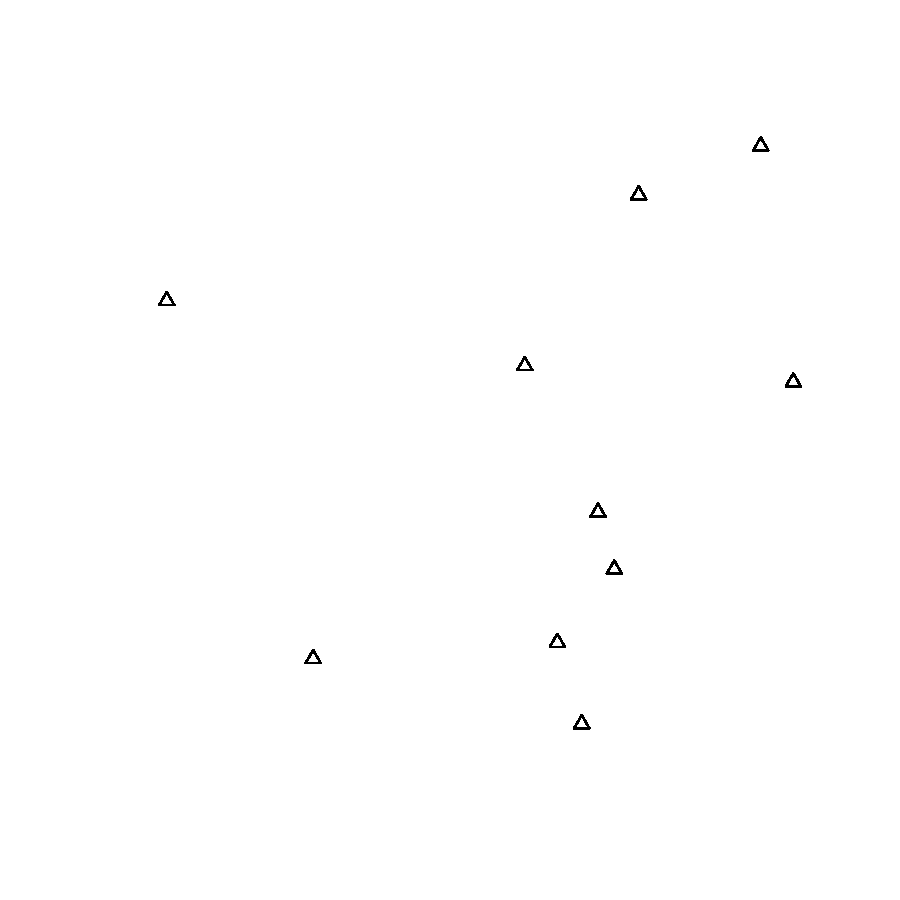
\includegraphics{sp-005}
\end{center}
\caption{plot of {\tt SpatialPoints} object; aspect ratio of x and y axis units is 1}
\label{fig:points}
\end{figure}

We can retrieve the coordinates from {\tt xy.sp} by
\begin{Schunk}
\begin{Sinput}
> xy.cc = coordinates(xy.sp)
> class(xy.cc)
\end{Sinput}
\begin{Soutput}
[1] "matrix"
\end{Soutput}
\begin{Sinput}
> dim(xy.cc)
\end{Sinput}
\begin{Soutput}
[1] 10  2
\end{Soutput}
\end{Schunk}
and other methods retrieve the bounding box, the dimensions, select points
(not dimensions or columns), coerce to a data.frame, or print a summary:
\begin{Schunk}
\begin{Sinput}
> bbox(xy.sp)
\end{Sinput}
\begin{Soutput}
    min  max
xc 0.19 0.96
yc 0.20 0.91
\end{Soutput}
\begin{Sinput}
> dimensions(xy.sp)
\end{Sinput}
\begin{Soutput}
[1] 2
\end{Soutput}
\begin{Sinput}
> xy.sp[1:2]
\end{Sinput}
\begin{Soutput}
SpatialPoints:
       xc   yc
[1,] 0.67 0.30
[2,] 0.96 0.62
Coordinate Reference System (CRS) arguments: NA 
\end{Soutput}
\begin{Sinput}
> xy.df = as.data.frame(xy.sp)
> class(xy.df)
\end{Sinput}
\begin{Soutput}
[1] "data.frame"
\end{Soutput}
\begin{Sinput}
> dim(xy.df)
\end{Sinput}
\begin{Soutput}
[1] 10  2
\end{Soutput}
\begin{Sinput}
> summary(xy.sp)
\end{Sinput}
\begin{Soutput}
Object of class SpatialPoints
Coordinates:
    min  max
xc 0.19 0.96
yc 0.20 0.91
Is projected: NA 
proj4string : [NA]
Number of points: 10
\end{Soutput}
\end{Schunk}

\subsection{Points with attributes}

One way of creating a {\tt SpatialPointsDataFrame} object is by building
it from a a {\tt SpatialPoints} object and a data.frame containing
the attributes:
\begin{Schunk}
\begin{Sinput}
> df = data.frame(z1 = round(5 + rnorm(10), 2), z2 = 20:29)
> df
\end{Sinput}
\begin{Soutput}
     z1 z2
1  3.10 20
2  4.15 21
3  3.68 22
4  4.45 23
5  6.62 24
6  5.57 25
7  3.66 26
8  3.75 27
9  5.19 28
10 5.02 29
\end{Soutput}
\begin{Sinput}
> xy.spdf = SpatialPointsDataFrame(xy.sp, df)
> xy.spdf
\end{Sinput}
\begin{Soutput}
    coordinates   z1 z2
1   (0.67, 0.3) 3.10 20
2  (0.96, 0.62) 4.15 21
3  (0.92, 0.91) 3.68 22
4  (0.77, 0.85) 4.45 23
5  (0.72, 0.46) 6.62 24
6  (0.74, 0.39) 5.57 25
7  (0.63, 0.64) 3.66 26
8  (0.19, 0.72) 3.75 27
9    (0.7, 0.2) 5.19 28
10 (0.37, 0.28) 5.02 29
\end{Soutput}
\begin{Sinput}
> summary(xy.spdf)
\end{Sinput}
\begin{Soutput}
Object of class SpatialPointsDataFrame
Coordinates:
    min  max
xc 0.19 0.96
yc 0.20 0.91
Is projected: NA 
proj4string : [NA]
Number of points: 10
Data attributes:
       z1              z2       
 Min.   :3.100   Min.   :20.00  
 1st Qu.:3.697   1st Qu.:22.25  
 Median :4.300   Median :24.50  
 Mean   :4.519   Mean   :24.50  
 3rd Qu.:5.147   3rd Qu.:26.75  
 Max.   :6.620   Max.   :29.00  
\end{Soutput}
\begin{Sinput}
> dimensions(xy.spdf)
\end{Sinput}
\begin{Soutput}
[1] 2
\end{Soutput}
\begin{Sinput}
> xy.spdf[1:2, ]
\end{Sinput}
\begin{Soutput}
   coordinates   z1 z2
1  (0.67, 0.3) 3.10 20
2 (0.96, 0.62) 4.15 21
\end{Soutput}
\begin{Sinput}
> xy.spdf[1]
\end{Sinput}
\begin{Soutput}
    coordinates   z1
1   (0.67, 0.3) 3.10
2  (0.96, 0.62) 4.15
3  (0.92, 0.91) 3.68
4  (0.77, 0.85) 4.45
5  (0.72, 0.46) 6.62
6  (0.74, 0.39) 5.57
7  (0.63, 0.64) 3.66
8  (0.19, 0.72) 3.75
9    (0.7, 0.2) 5.19
10 (0.37, 0.28) 5.02
\end{Soutput}
\begin{Sinput}
> xy.spdf[1:2, "z2"]
\end{Sinput}
\begin{Soutput}
   coordinates z2
1  (0.67, 0.3) 20
2 (0.96, 0.62) 21
\end{Soutput}
\begin{Sinput}
> xy.df = as.data.frame(xy.spdf)
> xy.df[1:2, ]
\end{Sinput}
\begin{Soutput}
    z1 z2   xc   yc
1 3.10 20 0.67 0.30
2 4.15 21 0.96 0.62
\end{Soutput}
\begin{Sinput}
> xy.cc = coordinates(xy.spdf)
> class(xy.cc)
\end{Sinput}
\begin{Soutput}
[1] "matrix"
\end{Soutput}
\begin{Sinput}
> dim(xy.cc)
\end{Sinput}
\begin{Soutput}
[1] 10  2
\end{Soutput}
\end{Schunk}
A note on selection with \verb|[|: the behaviour is as much as possible
copied from that of {\tt data.frame}s, but coordinates are always
sticky and allways a {\tt SpatialPointsDataFrame} is returned; {\tt
drop=FALSE} is not allowed. If coordinates should be dropped, use the
{\tt as.data.frame} method and select the non-coordinate data, or use
\verb|[[| to select a single attribute column (example below).

{\tt SpatialPointsDataFrame} objects can be created directly from 
data.frames by specifying which columns contain the coordinates:
\begin{Schunk}
\begin{Sinput}
> df1 = data.frame(xy, df)
> coordinates(df1) = c("xc", "yc")
> df1
\end{Sinput}
\begin{Soutput}
    coordinates   z1 z2
1   (0.67, 0.3) 3.10 20
2  (0.96, 0.62) 4.15 21
3  (0.92, 0.91) 3.68 22
4  (0.77, 0.85) 4.45 23
5  (0.72, 0.46) 6.62 24
6  (0.74, 0.39) 5.57 25
7  (0.63, 0.64) 3.66 26
8  (0.19, 0.72) 3.75 27
9    (0.7, 0.2) 5.19 28
10 (0.37, 0.28) 5.02 29
\end{Soutput}
\end{Schunk}
or
\begin{Schunk}
\begin{Sinput}
> df2 = data.frame(xy, df)
> coordinates(df2) = ~xc + yc
> df2[1:2, ]
\end{Sinput}
\begin{Soutput}
   coordinates   z1 z2
1  (0.67, 0.3) 3.10 20
2 (0.96, 0.62) 4.15 21
\end{Soutput}
\begin{Sinput}
> as.data.frame(df2)[1:2, ]
\end{Sinput}
\begin{Soutput}
    xc   yc   z1 z2
1 0.67 0.30 3.10 20
2 0.96 0.62 4.15 21
\end{Soutput}
\end{Schunk}
Note that in this form, {\tt coordinates} by setting (specifying) the
coordinates promotes its argument, an object of class {\tt data.frame}
to an object of class {\tt SpatialPointsDataFrame}. The method {\tt
as.data.frame} coerces back to the original {\tt data.frame}. When used
on a right-hand side of an equation, {\tt coordinates} {\em retrieves}
the matrix with coordinates:
\begin{Schunk}
\begin{Sinput}
> coordinates(df2)[1:2, ]
\end{Sinput}
\begin{Soutput}
       xc   yc
[1,] 0.67 0.30
[2,] 0.96 0.62
\end{Soutput}
\end{Schunk}
Elements (columns) in the data.frame part of an object can be manipulated
(retrieved, assigned) directly:
\begin{Schunk}
\begin{Sinput}
> df2[["z2"]]
\end{Sinput}
\begin{Soutput}
 [1] 20 21 22 23 24 25 26 27 28 29
\end{Soutput}
\begin{Sinput}
> df2[["z2"]][10] = 20
> df2[["z3"]] = 1:10
> summary(df2)
\end{Sinput}
\begin{Soutput}
Object of class SpatialPointsDataFrame
Coordinates:
    min  max
xc 0.19 0.96
yc 0.20 0.91
Is projected: NA 
proj4string : [NA]
Number of points: 10
Data attributes:
       z1              z2              z3       
 Min.   :3.100   Min.   :20.00   Min.   : 1.00  
 1st Qu.:3.697   1st Qu.:21.25   1st Qu.: 3.25  
 Median :4.300   Median :23.50   Median : 5.50  
 Mean   :4.519   Mean   :23.60   Mean   : 5.50  
 3rd Qu.:5.147   3rd Qu.:25.75   3rd Qu.: 7.75  
 Max.   :6.620   Max.   :28.00   Max.   :10.00  
\end{Soutput}
\end{Schunk}
Plotting attribute data can be done by using either {\tt spplot} to
colour symbols, or {\tt bubble} which uses symbol size:
\begin{Schunk}
\begin{Sinput}
> bubble(df2, "z1", key.space = "bottom")
> spplot(df2, "z1", key.space = "bottom")
\end{Sinput}
\end{Schunk}
the resulting plots are shown in figure \ref{fig:spdf}.

\begin{figure}
\begin{center}
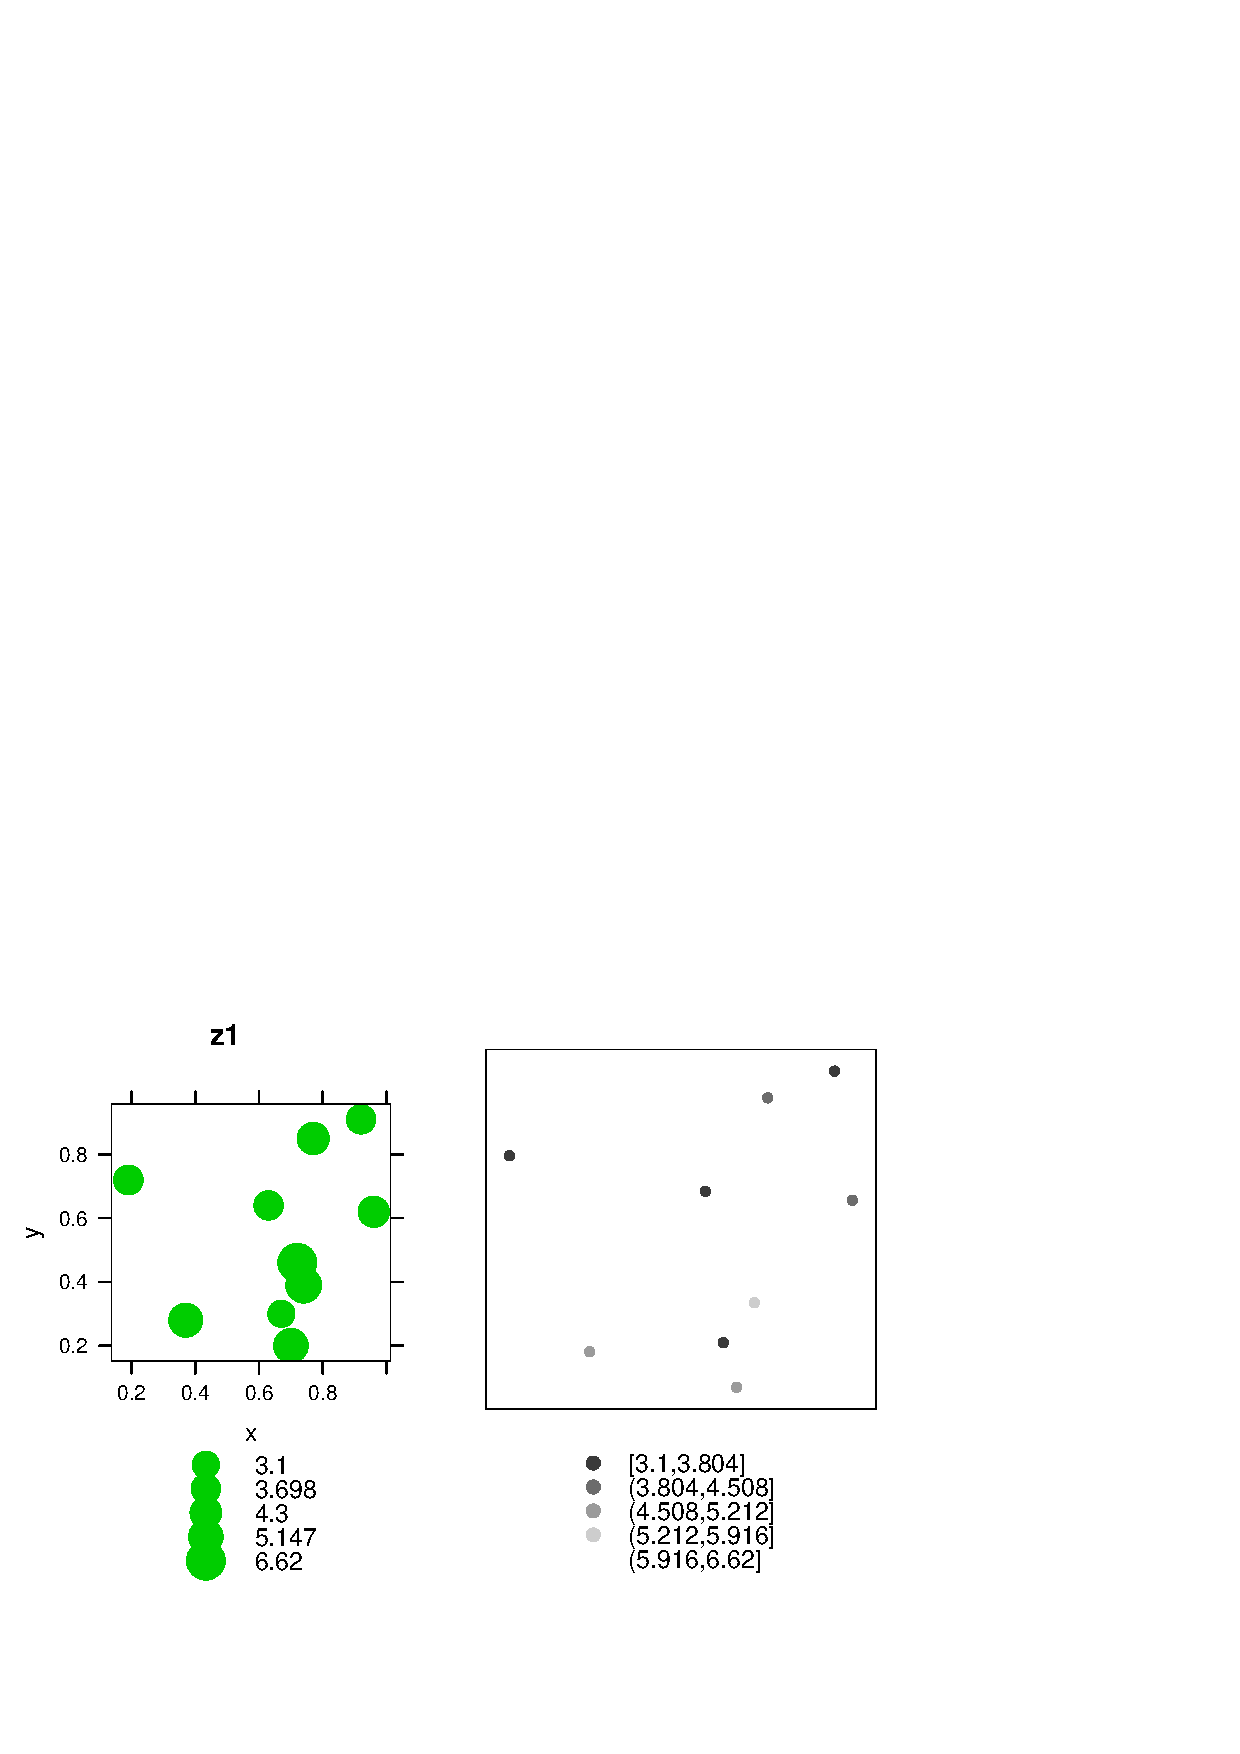
\includegraphics{sp-014}
\end{center}
\caption{plot of {\tt SpatialPointsDataFrame} object, using symbol 
size ({\tt bubble}, top) or colour ({\tt spplot}, bottom) }
\label{fig:spdf}
\end{figure}

\section{Grids}
Package {\tt sp} has two classes for grid topology: {\tt SpatialPixels}
and {\tt SpatialGrid}. The pixels form stores coordinates and is for
partial grids, or unordered points; the {\tt SpatialGrid} form does not
store coordinates but holds full grids (i.e., {\tt SpatialGridDataFrame}
holds attribute values for each grid cell). Objects can be coerced from
one representation to the other.

\subsection{Creating grids from topology}
When we know the offset, the cell sizes and the dimensions of a grid, we
can specify this by using the function {\tt GridTopology}:
\begin{Schunk}
\begin{Sinput}
> gt = GridTopology(cellcentre.offset = c(1, 1, 2), cellsize = c(1, 
+     1, 1), cells.dim = c(3, 4, 6))
> grd = SpatialGrid(gt)
> summary(grd)
\end{Sinput}
\begin{Soutput}
Object of class SpatialGrid
Coordinates:
          min max
coords.x1 0.5 3.5
coords.x2 0.5 4.5
coords.x3 1.5 7.5
Is projected: NA 
proj4string : [NA]
Number of points: 2
Grid attributes:
  cellcentre.offset cellsize cells.dim
1                 1        1         3
2                 1        1         4
3                 2        1         6
\end{Soutput}
\end{Schunk}

The grid parameters can be retrieved by the function
\begin{Schunk}
\begin{Sinput}
> gridparameters(grd)
\end{Sinput}
\begin{Soutput}
  cellcentre.offset cellsize cells.dim
1                 1        1         3
2                 1        1         4
3                 2        1         6
\end{Soutput}
\end{Schunk}

\subsection{Creating grids from points}
In the following example a three-dimensional grid is constructed from
a set of point coordinates:
\begin{Schunk}
\begin{Sinput}
> pts = expand.grid(x = 1:3, y = 1:4, z = 2:7)
> grd.pts = SpatialPixels(SpatialPoints(pts))
> summary(grd.pts)
\end{Sinput}
\begin{Soutput}
Object of class SpatialPixels
Coordinates:
  min max
x 0.5 3.5
y 0.5 4.5
z 1.5 7.5
Is projected: NA 
proj4string : [NA]
Number of points: 72
\end{Soutput}
\begin{Sinput}
> grd = as(grd.pts, "SpatialGrid")
> summary(grd)
\end{Sinput}
\begin{Soutput}
Object of class SpatialGrid
Coordinates:
  min max
x 0.5 3.5
y 0.5 4.5
z 1.5 7.5
Is projected: NA 
proj4string : [NA]
Number of points: 2
Grid attributes:
  cellcentre.offset cellsize cells.dim
x                 1        1         3
y                 1        1         4
z                 2        1         6
\end{Soutput}
\end{Schunk}
Note that when passed a points argument, SpatialPixels accepts a tolerance
(default 10 * .Machine\$double.eps) to specify how close the points have
to be to being exactly on a grid. For very large coordinates, this value
may have to be increased. A warning is issued if full rows and/or columns
are missing.

\subsection{Gridded data with attributes}

Spatial, gridded data are data with coordinates on a regular lattice.
To form such a grid we can go from coordinates:
\begin{Schunk}
\begin{Sinput}
> attr = expand.grid(xc = 1:3, yc = 1:3)
> grd.attr = data.frame(attr, z1 = 1:9, z2 = 9:1)
> coordinates(grd.attr) = ~xc + yc
> gridded(grd.attr)
\end{Sinput}
\begin{Soutput}
[1] FALSE
\end{Soutput}
\begin{Sinput}
> gridded(grd.attr) = TRUE
> gridded(grd.attr)
\end{Sinput}
\begin{Soutput}
[1] TRUE
\end{Soutput}
\begin{Sinput}
> summary(grd.attr)
\end{Sinput}
\begin{Soutput}
Object of class SpatialPixelsDataFrame
Coordinates:
   min max
xc 0.5 3.5
yc 0.5 3.5
Is projected: NA 
proj4string : [NA]
Number of points: 9
Data attributes:
       z1          z2   
 Min.   :1   Min.   :1  
 1st Qu.:3   1st Qu.:3  
 Median :5   Median :5  
 Mean   :5   Mean   :5  
 3rd Qu.:7   3rd Qu.:7  
 Max.   :9   Max.   :9  
\end{Soutput}
\end{Schunk}

\subsection{Are grids stored as points or as matrix/array?}

The form in which gridded data comes depends on whether the grid was
created from a set of points or from a matrix or external grid format
(e.g. read through rgdal). Retrieving the form, or conversion to another
can be done by {\tt as(x, "Class")}, or by using the function {\tt fullgrid}:
\begin{Schunk}
\begin{Sinput}
> fullgrid(grd)
\end{Sinput}
\begin{Soutput}
[1] TRUE
\end{Soutput}
\begin{Sinput}
> fullgrid(grd.pts)
\end{Sinput}
\begin{Soutput}
[1] FALSE
\end{Soutput}
\begin{Sinput}
> fullgrid(grd.attr)
\end{Sinput}
\begin{Soutput}
[1] FALSE
\end{Soutput}
\begin{Sinput}
> fullgrid(grd.pts) = TRUE
> fullgrid(grd.attr) = TRUE
> fullgrid(grd.pts)
\end{Sinput}
\begin{Soutput}
[1] TRUE
\end{Soutput}
\begin{Sinput}
> fullgrid(grd.attr)
\end{Sinput}
\begin{Soutput}
[1] TRUE
\end{Soutput}
\end{Schunk}

The advantage of having grids in cell form is that when a large part
of the grid contains missing values, these cells do not have to be
stored; also, no ordering of grid cells is required. For plotting by
a grid with {\tt levelplot}, this form is required and {\tt spplot}
(for grids a front-end to {\tt levelplot}) will convert grids that are
not in this form.  In contrast, {\tt image} requires a slightly altered
version of the the full grid form.  A disadvantage of the cell form is
that the coordinates for each point have to be stored, which may be
prohibitive for large grids.  Grids in cell form do have an index to
allow for fast transformation to the full grid form.

Besides {\tt print}, {\tt summary}, {\tt plot},
objects of class {\tt SpatialGridDataFrame} have methods for
\begin{itemize}
\item \verb|[| select rows (points) or columns (variables)
\item \verb|[[| retrieve a column from the attribute table (data.frame part)
\item \verb|[[<-| assign or replace a column in the attribute table (data.frame part)
\item {\tt coordinates} retrieve the coordinates of grid cells
\item {\tt as.matrix} retrieve the data as a matrix. The first index (rows) is the
x-column, the second index (columns) the y-coordinate. Row index 1 is the smallest
x-coordinate; column index 1 is the larges y-coordinate (top-to-bottom).
\item {\tt as} coercion methods for {\tt data.frame}, {\tt SpatialPointsDataFrame}
\item{\tt image} plot an image of the grid
\end{itemize}
Finally, {\tt spplot}, a front-end to {\tt levelplot} allows the
plotting of a single grid plot or a lattice of grid plots.

\subsection{Row and column selection of a region}
Rows/columns selection can be done when gridded data is in the full grid
form (as {\tt SpatialGridDataFrame}). In this form also rows and/or columns
can be de-selected (in which case a warning is issued):
\begin{Schunk}
\begin{Sinput}
> fullgrid(grd.attr) = FALSE
> grd.attr[1:5, "z1"]
\end{Sinput}
\begin{Soutput}
Object of class SpatialPixelsDataFrame
Object of class SpatialPixels
Grid topology:
   cellcentre.offset cellsize cells.dim
xc                 1        1         3
yc                 2        1         2
SpatialPoints:
     xc yc
[1,]  1  3
[2,]  2  3
[3,]  3  3
[4,]  1  2
[5,]  2  2
Coordinate Reference System (CRS) arguments: NA 

Data summary:
       z1     
 Min.   :4.0  
 1st Qu.:5.0  
 Median :7.0  
 Mean   :6.6  
 3rd Qu.:8.0  
 Max.   :9.0  
\end{Soutput}
\begin{Sinput}
> fullgrid(grd.attr) = TRUE
> grd.attr[1:2, -2, c("z2", "z1")]
\end{Sinput}
\begin{Soutput}
Object of class SpatialGridDataFrame
Object of class SpatialGrid
Grid topology:
   cellcentre.offset cellsize cells.dim
xc                 1        2         2
yc                 2        1         2
SpatialPoints:
     xc yc
[1,]  1  3
[2,]  3  3
[3,]  1  2
[4,]  3  2
Coordinate Reference System (CRS) arguments: NA 

Data summary:
       z2            z1     
 Min.   :1.0   Min.   :4.0  
 1st Qu.:2.5   1st Qu.:5.5  
 Median :3.5   Median :6.5  
 Mean   :3.5   Mean   :6.5  
 3rd Qu.:4.5   3rd Qu.:7.5  
 Max.   :6.0   Max.   :9.0  
\end{Soutput}
\end{Schunk}

\section{Lines}

\subsection{Building line objects from scratch}
In many instances, line coordinates will be retrieved from external
sources.  The following example shows how to build an object of class
{\tt SpatialLines} from scratch. Note that the {\tt Lines} objects have to be given character ID values, and that these values must be unique for {\tt Lines} objects combined in a {\tt SpatialLines} object.

% build line objects
\begin{Schunk}
\begin{Sinput}
> l1 = cbind(c(1, 2, 3), c(3, 2, 2))
> l1a = cbind(l1[, 1] + 0.05, l1[, 2] + 0.05)
> l2 = cbind(c(1, 2, 3), c(1, 1.5, 1))
> Sl1 = Line(l1)
> Sl1a = Line(l1a)
> Sl2 = Line(l2)
> S1 = Lines(list(Sl1, Sl1a), ID = "a")
> S2 = Lines(list(Sl2), ID = "b")
> Sl = SpatialLines(list(S1, S2))
> summary(Sl)
\end{Sinput}
\begin{Soutput}
Object of class SpatialLines
Coordinates:
   min max
r1   1   3
r2   1   3
Is projected: NA 
proj4string : [NA]
\end{Soutput}
\begin{Sinput}
> plot(Sl, col = c("red", "blue"))
\end{Sinput}
\end{Schunk}
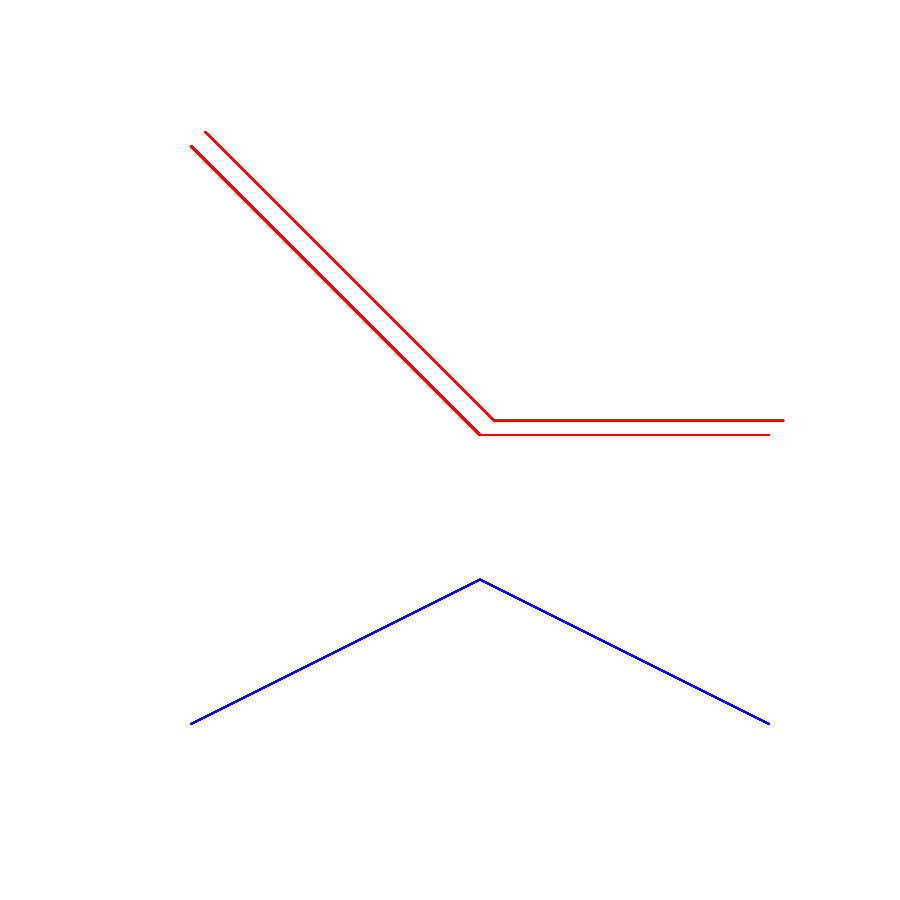
\includegraphics{sp-021}

\subsection{Building line objects with attributes}

The class {\tt SpatialLinesDataFrame} is designed for holding
lines data that have an attribute table (data.frame) attached
to it:
\begin{Schunk}
\begin{Sinput}
> df = data.frame(z = c(1, 2), row.names = getSLLinesIDSlots(Sl))
> Sldf = SpatialLinesDataFrame(Sl, data = df)
> summary(Sldf)
\end{Sinput}
\begin{Soutput}
Object of class SpatialLinesDataFrame
Coordinates:
   min max
r1   1   3
r2   1   3
Is projected: NA 
proj4string : [NA]
Data attributes:
       z       
 Min.   :1.00  
 1st Qu.:1.25  
 Median :1.50  
 Mean   :1.50  
 3rd Qu.:1.75  
 Max.   :2.00  
\end{Soutput}
\end{Schunk}
Not many useful methods for it are available yet.  The {\tt plot} method
only plots the lines, ignoring attribute table values. Suggestions for
useful methods are welcome.

\section{Polygons}

\subsection{Building from scratch}
The following example shows how a set of polygons are built from scratch.
Note that {\tt Sr4} has the opposite direction (anti-clockwise) as the other three (clockwise);
it is meant to represent a hole in the {\tt Sr3} polygon. The default value for the hole colour {\tt pbg} is {\tt "transparent}, which will not show, but which often does not matter, because another polygon fills the hole --- here it is set to {\tt "white"}. Note that the {\tt Polygons} objects have to be given character ID values, and that these values must be unique for {\tt Polygons} objects combined in a {\tt SpatialPolygons} object.
\begin{Schunk}
\begin{Sinput}
> Sr1 = Polygon(cbind(c(2, 4, 4, 1, 2), c(2, 3, 5, 4, 2)))
> Sr2 = Polygon(cbind(c(5, 4, 2, 5), c(2, 3, 2, 2)))
> Sr3 = Polygon(cbind(c(4, 4, 5, 10, 4), c(5, 3, 2, 5, 5)))
> Sr4 = Polygon(cbind(c(5, 6, 6, 5, 5), c(4, 4, 3, 3, 4)), hole = TRUE)
> Srs1 = Polygons(list(Sr1), "s1")
> Srs2 = Polygons(list(Sr2), "s2")
> Srs3 = Polygons(list(Sr3, Sr4), "s3/4")
> SpP = SpatialPolygons(list(Srs1, Srs2, Srs3), 1:3)
> plot(SpP, col = 1:3, pbg = "white")
\end{Sinput}
\end{Schunk}
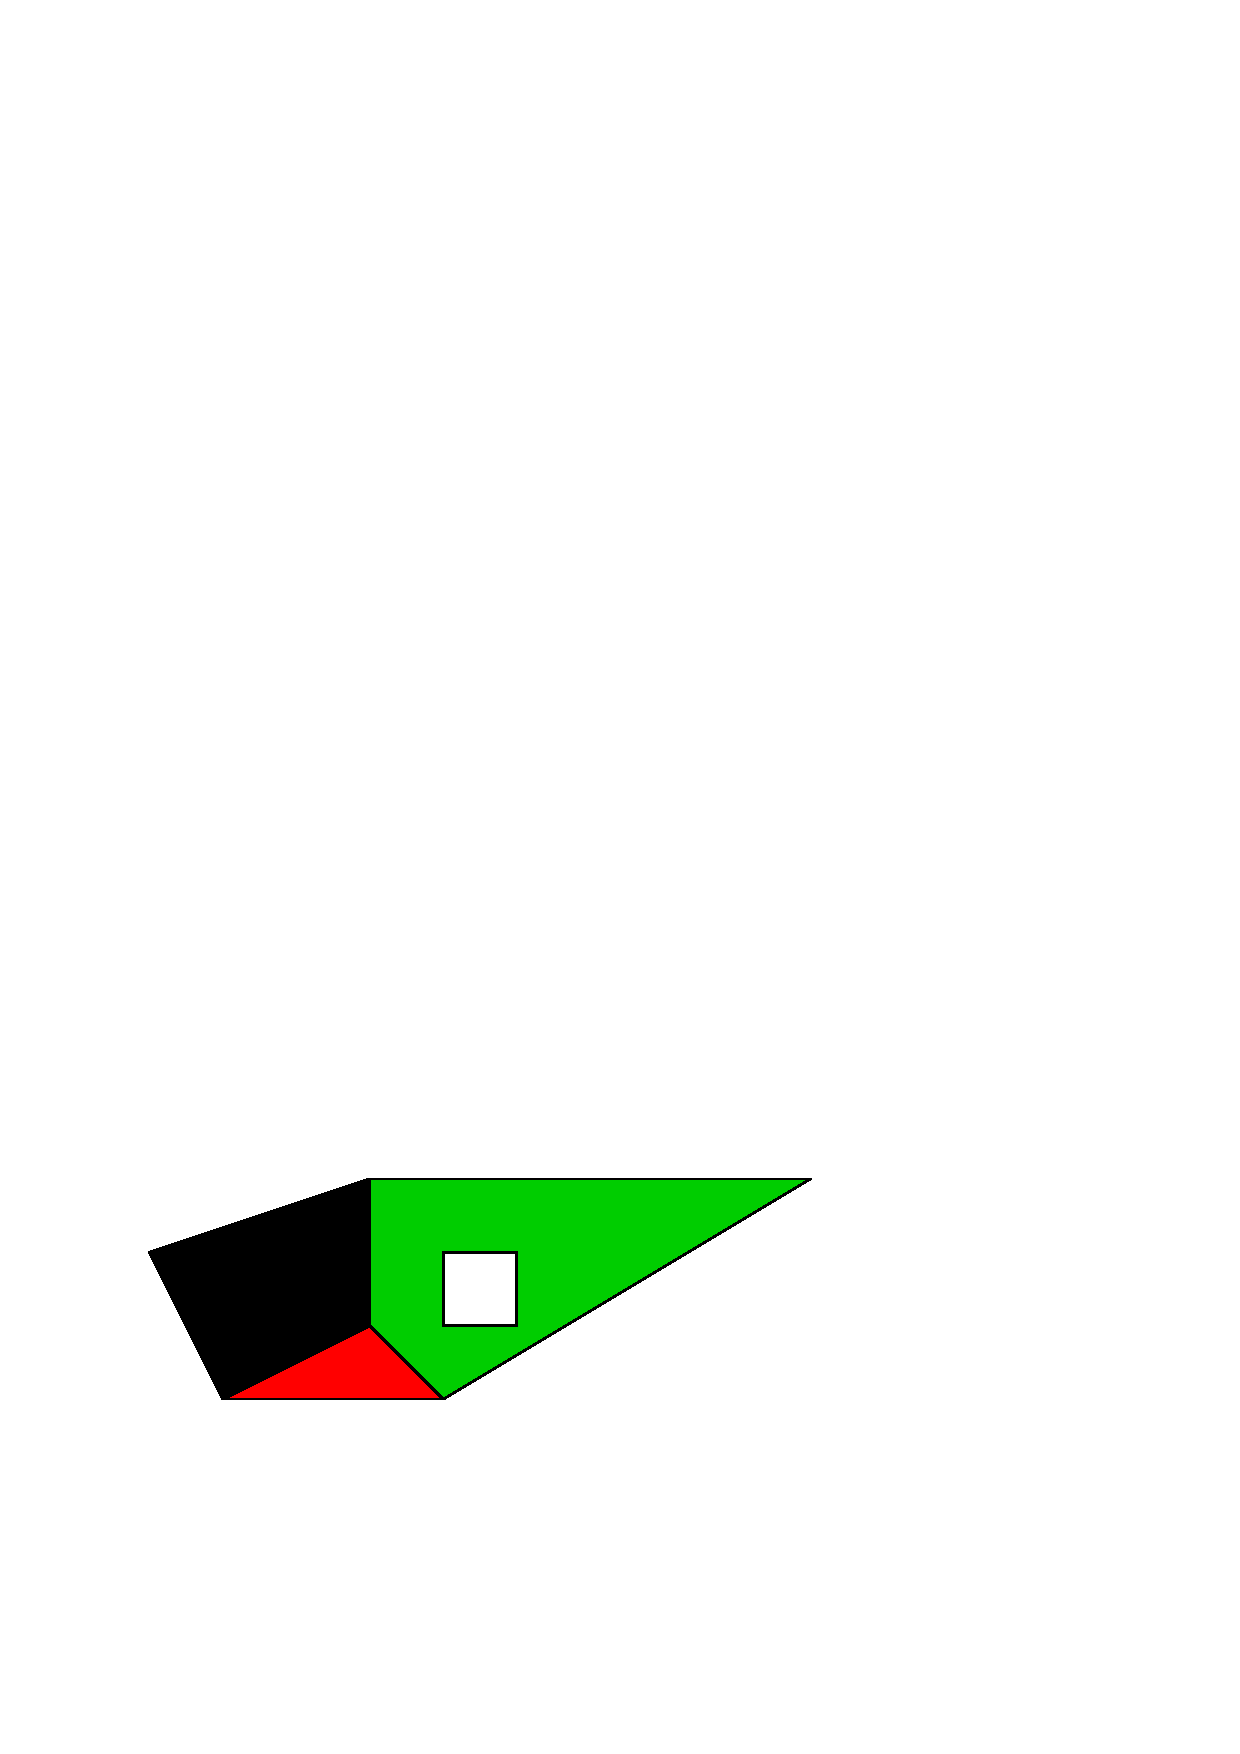
\includegraphics{sp-023}

\subsection{Polygons with attributes}
Polygons with attributes, objects of class {\tt SpatialPolygonsDataFrame},
are built from the {\tt SpatialPolygons} object (topology) and the attributes
(data.frame). The {\tt row.names} of the attributes data frame are matched with the ID slots of the {\tt SpatialPolygons} object, and the rows of the data frame will be re-ordered if necessary.
\begin{Schunk}
\begin{Sinput}
> attr = data.frame(a = 1:3, b = 3:1, row.names = c("s3/4", "s2", 
+     "s1"))
> SrDf = SpatialPolygonsDataFrame(SpP, attr)
> as(SrDf, "data.frame")
\end{Sinput}
\begin{Soutput}
     a b
s1   3 1
s2   2 2
s3/4 1 3
\end{Soutput}
\begin{Sinput}
> spplot(SrDf)
\end{Sinput}
\end{Schunk}

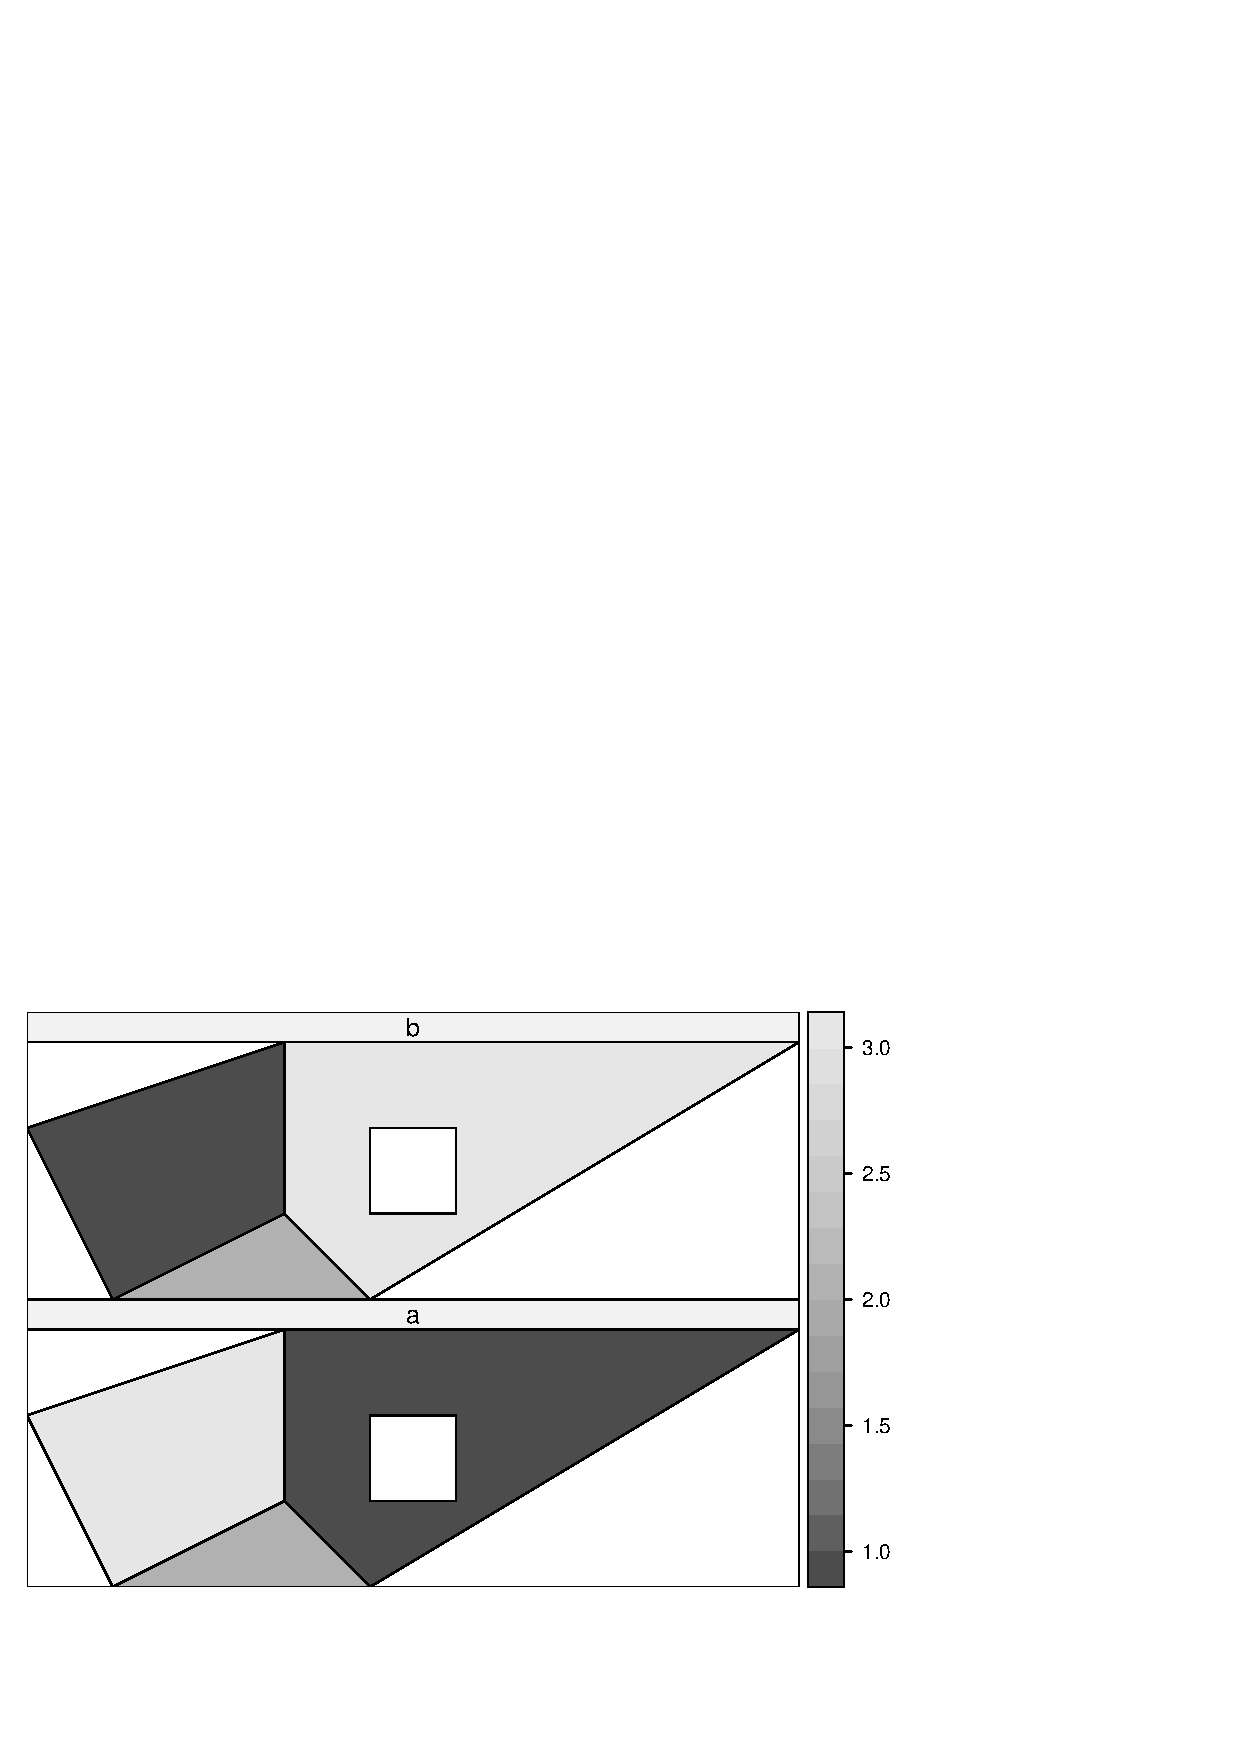
\includegraphics{sp-025}

or, as another way to create the {\tt SpatialPolygonsDataFrame} object:
\begin{Schunk}
\begin{Sinput}
> SrDf = attr
> polygons(SrDf) = SpP
\end{Sinput}
\end{Schunk}

\section{Importing and exporting data}

Data import and export from external data sources and file formats
is handled inthe \pkg{rgdal} package in the first instance, using the
available OGR/GDAL drivers for vector and raster data. This keeps the
range of drivers up to date, and secures code maintenance through working
closely with the open source geospatial community. Mac OSX users unable
or unwilling to install \pkg{rgdal} from source after installing its
external dependencies will find some functions in the \pkg{maptools}
package to import and export a limited range of formats.


\section*{References}
\begin{description}
\item Chambers, J.M., 1998, Programming with data, a guide to the S language.
Springer, New York.
\end{description}

\end{document}

% vim:syntax=tex
